\documentclass{article} % For LaTeX2e
\usepackage{iclr2022_conference,times}
% Optional math commands from https://github.com/goodfeli/dlbook_notation.
%%%%% NEW MATH DEFINITIONS %%%%%

\usepackage{amsmath,amsfonts,bm}

% Mark sections of captions for referring to divisions of figures
\newcommand{\figleft}{{\em (Left)}}
\newcommand{\figcenter}{{\em (Center)}}
\newcommand{\figright}{{\em (Right)}}
\newcommand{\figtop}{{\em (Top)}}
\newcommand{\figbottom}{{\em (Bottom)}}
\newcommand{\captiona}{{\em (a)}}
\newcommand{\captionb}{{\em (b)}}
\newcommand{\captionc}{{\em (c)}}
\newcommand{\captiond}{{\em (d)}}

% Highlight a newly defined term
\newcommand{\newterm}[1]{{\bf #1}}


% Figure reference, lower-case.
\def\figref#1{figure~\ref{#1}}
% Figure reference, capital. For start of sentence
\def\Figref#1{Figure~\ref{#1}}
\def\twofigref#1#2{figures \ref{#1} and \ref{#2}}
\def\quadfigref#1#2#3#4{figures \ref{#1}, \ref{#2}, \ref{#3} and \ref{#4}}
% Section reference, lower-case.
\def\secref#1{section~\ref{#1}}
% Section reference, capital.
\def\Secref#1{Section~\ref{#1}}
% Reference to two sections.
\def\twosecrefs#1#2{sections \ref{#1} and \ref{#2}}
% Reference to three sections.
\def\secrefs#1#2#3{sections \ref{#1}, \ref{#2} and \ref{#3}}
% Reference to an equation, lower-case.
\def\eqref#1{equation~\ref{#1}}
% Reference to an equation, upper case
\def\Eqref#1{Equation~\ref{#1}}
% A raw reference to an equation---avoid using if possible
\def\plaineqref#1{\ref{#1}}
% Reference to a chapter, lower-case.
\def\chapref#1{chapter~\ref{#1}}
% Reference to an equation, upper case.
\def\Chapref#1{Chapter~\ref{#1}}
% Reference to a range of chapters
\def\rangechapref#1#2{chapters\ref{#1}--\ref{#2}}
% Reference to an algorithm, lower-case.
\def\algref#1{algorithm~\ref{#1}}
% Reference to an algorithm, upper case.
\def\Algref#1{Algorithm~\ref{#1}}
\def\twoalgref#1#2{algorithms \ref{#1} and \ref{#2}}
\def\Twoalgref#1#2{Algorithms \ref{#1} and \ref{#2}}
% Reference to a part, lower case
\def\partref#1{part~\ref{#1}}
% Reference to a part, upper case
\def\Partref#1{Part~\ref{#1}}
\def\twopartref#1#2{parts \ref{#1} and \ref{#2}}

\def\ceil#1{\lceil #1 \rceil}
\def\floor#1{\lfloor #1 \rfloor}
\def\1{\bm{1}}
\newcommand{\train}{\mathcal{D}}
\newcommand{\valid}{\mathcal{D_{\mathrm{valid}}}}
\newcommand{\test}{\mathcal{D_{\mathrm{test}}}}

\def\eps{{\epsilon}}


% Random variables
\def\reta{{\textnormal{$\eta$}}}
\def\ra{{\textnormal{a}}}
\def\rb{{\textnormal{b}}}
\def\rc{{\textnormal{c}}}
\def\rd{{\textnormal{d}}}
\def\re{{\textnormal{e}}}
\def\rf{{\textnormal{f}}}
\def\rg{{\textnormal{g}}}
\def\rh{{\textnormal{h}}}
\def\ri{{\textnormal{i}}}
\def\rj{{\textnormal{j}}}
\def\rk{{\textnormal{k}}}
\def\rl{{\textnormal{l}}}
% rm is already a command, just don't name any random variables m
\def\rn{{\textnormal{n}}}
\def\ro{{\textnormal{o}}}
\def\rp{{\textnormal{p}}}
\def\rq{{\textnormal{q}}}
\def\rr{{\textnormal{r}}}
\def\rs{{\textnormal{s}}}
\def\rt{{\textnormal{t}}}
\def\ru{{\textnormal{u}}}
\def\rv{{\textnormal{v}}}
\def\rw{{\textnormal{w}}}
\def\rx{{\textnormal{x}}}
\def\ry{{\textnormal{y}}}
\def\rz{{\textnormal{z}}}

% Random vectors
\def\rvepsilon{{\mathbf{\epsilon}}}
\def\rvtheta{{\mathbf{\theta}}}
\def\rva{{\mathbf{a}}}
\def\rvb{{\mathbf{b}}}
\def\rvc{{\mathbf{c}}}
\def\rvd{{\mathbf{d}}}
\def\rve{{\mathbf{e}}}
\def\rvf{{\mathbf{f}}}
\def\rvg{{\mathbf{g}}}
\def\rvh{{\mathbf{h}}}
\def\rvu{{\mathbf{i}}}
\def\rvj{{\mathbf{j}}}
\def\rvk{{\mathbf{k}}}
\def\rvl{{\mathbf{l}}}
\def\rvm{{\mathbf{m}}}
\def\rvn{{\mathbf{n}}}
\def\rvo{{\mathbf{o}}}
\def\rvp{{\mathbf{p}}}
\def\rvq{{\mathbf{q}}}
\def\rvr{{\mathbf{r}}}
\def\rvs{{\mathbf{s}}}
\def\rvt{{\mathbf{t}}}
\def\rvu{{\mathbf{u}}}
\def\rvv{{\mathbf{v}}}
\def\rvw{{\mathbf{w}}}
\def\rvx{{\mathbf{x}}}
\def\rvy{{\mathbf{y}}}
\def\rvz{{\mathbf{z}}}

% Elements of random vectors
\def\erva{{\textnormal{a}}}
\def\ervb{{\textnormal{b}}}
\def\ervc{{\textnormal{c}}}
\def\ervd{{\textnormal{d}}}
\def\erve{{\textnormal{e}}}
\def\ervf{{\textnormal{f}}}
\def\ervg{{\textnormal{g}}}
\def\ervh{{\textnormal{h}}}
\def\ervi{{\textnormal{i}}}
\def\ervj{{\textnormal{j}}}
\def\ervk{{\textnormal{k}}}
\def\ervl{{\textnormal{l}}}
\def\ervm{{\textnormal{m}}}
\def\ervn{{\textnormal{n}}}
\def\ervo{{\textnormal{o}}}
\def\ervp{{\textnormal{p}}}
\def\ervq{{\textnormal{q}}}
\def\ervr{{\textnormal{r}}}
\def\ervs{{\textnormal{s}}}
\def\ervt{{\textnormal{t}}}
\def\ervu{{\textnormal{u}}}
\def\ervv{{\textnormal{v}}}
\def\ervw{{\textnormal{w}}}
\def\ervx{{\textnormal{x}}}
\def\ervy{{\textnormal{y}}}
\def\ervz{{\textnormal{z}}}

% Random matrices
\def\rmA{{\mathbf{A}}}
\def\rmB{{\mathbf{B}}}
\def\rmC{{\mathbf{C}}}
\def\rmD{{\mathbf{D}}}
\def\rmE{{\mathbf{E}}}
\def\rmF{{\mathbf{F}}}
\def\rmG{{\mathbf{G}}}
\def\rmH{{\mathbf{H}}}
\def\rmI{{\mathbf{I}}}
\def\rmJ{{\mathbf{J}}}
\def\rmK{{\mathbf{K}}}
\def\rmL{{\mathbf{L}}}
\def\rmM{{\mathbf{M}}}
\def\rmN{{\mathbf{N}}}
\def\rmO{{\mathbf{O}}}
\def\rmP{{\mathbf{P}}}
\def\rmQ{{\mathbf{Q}}}
\def\rmR{{\mathbf{R}}}
\def\rmS{{\mathbf{S}}}
\def\rmT{{\mathbf{T}}}
\def\rmU{{\mathbf{U}}}
\def\rmV{{\mathbf{V}}}
\def\rmW{{\mathbf{W}}}
\def\rmX{{\mathbf{X}}}
\def\rmY{{\mathbf{Y}}}
\def\rmZ{{\mathbf{Z}}}

% Elements of random matrices
\def\ermA{{\textnormal{A}}}
\def\ermB{{\textnormal{B}}}
\def\ermC{{\textnormal{C}}}
\def\ermD{{\textnormal{D}}}
\def\ermE{{\textnormal{E}}}
\def\ermF{{\textnormal{F}}}
\def\ermG{{\textnormal{G}}}
\def\ermH{{\textnormal{H}}}
\def\ermI{{\textnormal{I}}}
\def\ermJ{{\textnormal{J}}}
\def\ermK{{\textnormal{K}}}
\def\ermL{{\textnormal{L}}}
\def\ermM{{\textnormal{M}}}
\def\ermN{{\textnormal{N}}}
\def\ermO{{\textnormal{O}}}
\def\ermP{{\textnormal{P}}}
\def\ermQ{{\textnormal{Q}}}
\def\ermR{{\textnormal{R}}}
\def\ermS{{\textnormal{S}}}
\def\ermT{{\textnormal{T}}}
\def\ermU{{\textnormal{U}}}
\def\ermV{{\textnormal{V}}}
\def\ermW{{\textnormal{W}}}
\def\ermX{{\textnormal{X}}}
\def\ermY{{\textnormal{Y}}}
\def\ermZ{{\textnormal{Z}}}

% Vectors
\def\vzero{{\bm{0}}}
\def\vone{{\bm{1}}}
\def\vmu{{\bm{\mu}}}
\def\vtheta{{\bm{\theta}}}
\def\va{{\bm{a}}}
\def\vb{{\bm{b}}}
\def\vc{{\bm{c}}}
\def\vd{{\bm{d}}}
\def\ve{{\bm{e}}}
\def\vf{{\bm{f}}}
\def\vg{{\bm{g}}}
\def\vh{{\bm{h}}}
\def\vi{{\bm{i}}}
\def\vj{{\bm{j}}}
\def\vk{{\bm{k}}}
\def\vl{{\bm{l}}}
\def\vm{{\bm{m}}}
\def\vn{{\bm{n}}}
\def\vo{{\bm{o}}}
\def\vp{{\bm{p}}}
\def\vq{{\bm{q}}}
\def\vr{{\bm{r}}}
\def\vs{{\bm{s}}}
\def\vt{{\bm{t}}}
\def\vu{{\bm{u}}}
\def\vv{{\bm{v}}}
\def\vw{{\bm{w}}}
\def\vx{{\bm{x}}}
\def\vy{{\bm{y}}}
\def\vz{{\bm{z}}}

% Elements of vectors
\def\evalpha{{\alpha}}
\def\evbeta{{\beta}}
\def\evepsilon{{\epsilon}}
\def\evlambda{{\lambda}}
\def\evomega{{\omega}}
\def\evmu{{\mu}}
\def\evpsi{{\psi}}
\def\evsigma{{\sigma}}
\def\evtheta{{\theta}}
\def\eva{{a}}
\def\evb{{b}}
\def\evc{{c}}
\def\evd{{d}}
\def\eve{{e}}
\def\evf{{f}}
\def\evg{{g}}
\def\evh{{h}}
\def\evi{{i}}
\def\evj{{j}}
\def\evk{{k}}
\def\evl{{l}}
\def\evm{{m}}
\def\evn{{n}}
\def\evo{{o}}
\def\evp{{p}}
\def\evq{{q}}
\def\evr{{r}}
\def\evs{{s}}
\def\evt{{t}}
\def\evu{{u}}
\def\evv{{v}}
\def\evw{{w}}
\def\evx{{x}}
\def\evy{{y}}
\def\evz{{z}}

% Matrix
\def\mA{{\bm{A}}}
\def\mB{{\bm{B}}}
\def\mC{{\bm{C}}}
\def\mD{{\bm{D}}}
\def\mE{{\bm{E}}}
\def\mF{{\bm{F}}}
\def\mG{{\bm{G}}}
\def\mH{{\bm{H}}}
\def\mI{{\bm{I}}}
\def\mJ{{\bm{J}}}
\def\mK{{\bm{K}}}
\def\mL{{\bm{L}}}
\def\mM{{\bm{M}}}
\def\mN{{\bm{N}}}
\def\mO{{\bm{O}}}
\def\mP{{\bm{P}}}
\def\mQ{{\bm{Q}}}
\def\mR{{\bm{R}}}
\def\mS{{\bm{S}}}
\def\mT{{\bm{T}}}
\def\mU{{\bm{U}}}
\def\mV{{\bm{V}}}
\def\mW{{\bm{W}}}
\def\mX{{\bm{X}}}
\def\mY{{\bm{Y}}}
\def\mZ{{\bm{Z}}}
\def\mBeta{{\bm{\beta}}}
\def\mPhi{{\bm{\Phi}}}
\def\mLambda{{\bm{\Lambda}}}
\def\mSigma{{\bm{\Sigma}}}

% Tensor
\DeclareMathAlphabet{\mathsfit}{\encodingdefault}{\sfdefault}{m}{sl}
\SetMathAlphabet{\mathsfit}{bold}{\encodingdefault}{\sfdefault}{bx}{n}
\newcommand{\tens}[1]{\bm{\mathsfit{#1}}}
\def\tA{{\tens{A}}}
\def\tB{{\tens{B}}}
\def\tC{{\tens{C}}}
\def\tD{{\tens{D}}}
\def\tE{{\tens{E}}}
\def\tF{{\tens{F}}}
\def\tG{{\tens{G}}}
\def\tH{{\tens{H}}}
\def\tI{{\tens{I}}}
\def\tJ{{\tens{J}}}
\def\tK{{\tens{K}}}
\def\tL{{\tens{L}}}
\def\tM{{\tens{M}}}
\def\tN{{\tens{N}}}
\def\tO{{\tens{O}}}
\def\tP{{\tens{P}}}
\def\tQ{{\tens{Q}}}
\def\tR{{\tens{R}}}
\def\tS{{\tens{S}}}
\def\tT{{\tens{T}}}
\def\tU{{\tens{U}}}
\def\tV{{\tens{V}}}
\def\tW{{\tens{W}}}
\def\tX{{\tens{X}}}
\def\tY{{\tens{Y}}}
\def\tZ{{\tens{Z}}}


% Graph
\def\gA{{\mathcal{A}}}
\def\gB{{\mathcal{B}}}
\def\gC{{\mathcal{C}}}
\def\gD{{\mathcal{D}}}
\def\gE{{\mathcal{E}}}
\def\gF{{\mathcal{F}}}
\def\gG{{\mathcal{G}}}
\def\gH{{\mathcal{H}}}
\def\gI{{\mathcal{I}}}
\def\gJ{{\mathcal{J}}}
\def\gK{{\mathcal{K}}}
\def\gL{{\mathcal{L}}}
\def\gM{{\mathcal{M}}}
\def\gN{{\mathcal{N}}}
\def\gO{{\mathcal{O}}}
\def\gP{{\mathcal{P}}}
\def\gQ{{\mathcal{Q}}}
\def\gR{{\mathcal{R}}}
\def\gS{{\mathcal{S}}}
\def\gT{{\mathcal{T}}}
\def\gU{{\mathcal{U}}}
\def\gV{{\mathcal{V}}}
\def\gW{{\mathcal{W}}}
\def\gX{{\mathcal{X}}}
\def\gY{{\mathcal{Y}}}
\def\gZ{{\mathcal{Z}}}

% Sets
\def\sA{{\mathbb{A}}}
\def\sB{{\mathbb{B}}}
\def\sC{{\mathbb{C}}}
\def\sD{{\mathbb{D}}}
% Don't use a set called E, because this would be the same as our symbol
% for expectation.
\def\sF{{\mathbb{F}}}
\def\sG{{\mathbb{G}}}
\def\sH{{\mathbb{H}}}
\def\sI{{\mathbb{I}}}
\def\sJ{{\mathbb{J}}}
\def\sK{{\mathbb{K}}}
\def\sL{{\mathbb{L}}}
\def\sM{{\mathbb{M}}}
\def\sN{{\mathbb{N}}}
\def\sO{{\mathbb{O}}}
\def\sP{{\mathbb{P}}}
\def\sQ{{\mathbb{Q}}}
\def\sR{{\mathbb{R}}}
\def\sS{{\mathbb{S}}}
\def\sT{{\mathbb{T}}}
\def\sU{{\mathbb{U}}}
\def\sV{{\mathbb{V}}}
\def\sW{{\mathbb{W}}}
\def\sX{{\mathbb{X}}}
\def\sY{{\mathbb{Y}}}
\def\sZ{{\mathbb{Z}}}

% Entries of a matrix
\def\emLambda{{\Lambda}}
\def\emA{{A}}
\def\emB{{B}}
\def\emC{{C}}
\def\emD{{D}}
\def\emE{{E}}
\def\emF{{F}}
\def\emG{{G}}
\def\emH{{H}}
\def\emI{{I}}
\def\emJ{{J}}
\def\emK{{K}}
\def\emL{{L}}
\def\emM{{M}}
\def\emN{{N}}
\def\emO{{O}}
\def\emP{{P}}
\def\emQ{{Q}}
\def\emR{{R}}
\def\emS{{S}}
\def\emT{{T}}
\def\emU{{U}}
\def\emV{{V}}
\def\emW{{W}}
\def\emX{{X}}
\def\emY{{Y}}
\def\emZ{{Z}}
\def\emSigma{{\Sigma}}

% entries of a tensor
% Same font as tensor, without \bm wrapper
\newcommand{\etens}[1]{\mathsfit{#1}}
\def\etLambda{{\etens{\Lambda}}}
\def\etA{{\etens{A}}}
\def\etB{{\etens{B}}}
\def\etC{{\etens{C}}}
\def\etD{{\etens{D}}}
\def\etE{{\etens{E}}}
\def\etF{{\etens{F}}}
\def\etG{{\etens{G}}}
\def\etH{{\etens{H}}}
\def\etI{{\etens{I}}}
\def\etJ{{\etens{J}}}
\def\etK{{\etens{K}}}
\def\etL{{\etens{L}}}
\def\etM{{\etens{M}}}
\def\etN{{\etens{N}}}
\def\etO{{\etens{O}}}
\def\etP{{\etens{P}}}
\def\etQ{{\etens{Q}}}
\def\etR{{\etens{R}}}
\def\etS{{\etens{S}}}
\def\etT{{\etens{T}}}
\def\etU{{\etens{U}}}
\def\etV{{\etens{V}}}
\def\etW{{\etens{W}}}
\def\etX{{\etens{X}}}
\def\etY{{\etens{Y}}}
\def\etZ{{\etens{Z}}}

% The true underlying data generating distribution
\newcommand{\pdata}{p_{\rm{data}}}
% The empirical distribution defined by the training set
\newcommand{\ptrain}{\hat{p}_{\rm{data}}}
\newcommand{\Ptrain}{\hat{P}_{\rm{data}}}
% The model distribution
\newcommand{\pmodel}{p_{\rm{model}}}
\newcommand{\Pmodel}{P_{\rm{model}}}
\newcommand{\ptildemodel}{\tilde{p}_{\rm{model}}}
% Stochastic autoencoder distributions
\newcommand{\pencode}{p_{\rm{encoder}}}
\newcommand{\pdecode}{p_{\rm{decoder}}}
\newcommand{\precons}{p_{\rm{reconstruct}}}

\newcommand{\laplace}{\mathrm{Laplace}} % Laplace distribution

\newcommand{\E}{\mathbb{E}}
\newcommand{\Ls}{\mathcal{L}}
\newcommand{\R}{\mathbb{R}}
\newcommand{\emp}{\tilde{p}}
\newcommand{\lr}{\alpha}
\newcommand{\reg}{\lambda}
\newcommand{\rect}{\mathrm{rectifier}}
\newcommand{\softmax}{\mathrm{softmax}}
\newcommand{\sigmoid}{\sigma}
\newcommand{\softplus}{\zeta}
\newcommand{\KL}{D_{\mathrm{KL}}}
\newcommand{\Var}{\mathrm{Var}}
\newcommand{\standarderror}{\mathrm{SE}}
\newcommand{\Cov}{\mathrm{Cov}}
% Wolfram Mathworld says $L^2$ is for function spaces and $\ell^2$ is for vectors
% But then they seem to use $L^2$ for vectors throughout the site, and so does
% wikipedia.
\newcommand{\normlzero}{L^0}
\newcommand{\normlone}{L^1}
\newcommand{\normltwo}{L^2}
\newcommand{\normlp}{L^p}
\newcommand{\normmax}{L^\infty}

\newcommand{\parents}{Pa} % See usage in notation.tex. Chosen to match Daphne's book.

\DeclareMathOperator*{\argmax}{arg\,max}
\DeclareMathOperator*{\argmin}{arg\,min}

\DeclareMathOperator{\sign}{sign}
\DeclareMathOperator{\Tr}{Tr}
\let\ab\allowbreak


%######## APS360: Uncomment your submission name
\newcommand{\apsname}{Project Proposal}
%\newcommand{\apsname}{Progress Report}
%\newcommand{\apsname}{Final Report}

%######## APS360: Put your Group Number here
\newcommand{\gpnumber}{28}

\usepackage{hyperref}
\usepackage{url}
\usepackage{graphicx}


%######## APS360: Put your project Title here
\title{Project Proposal: Traffic Sign Recognition Through Deep Learning}


%######## APS360: Put your names, student IDs and Emails here
\author{Salwa Waseem  \\
Student\# 10090214161\\
\texttt{salwa.waseem@mail.utoronto.ca} \\
\And
Maya Ramaneetharan Ramanathan  \\
Student\# 1008717596 \\
\texttt{maya.ramanathan@mail.utoronto.ca} \\
\AND
Maryah Noorani  \\
Student\# 1008343188 \\
\texttt{maryah.noorani@mail.utoronto.ca} \\
\And
Seoyeon (Sally) Kim \\
Student\# 1007713949 \\
\texttt{sysally.kim@@mail.utoronto.ca} \\
\AND
}

% The \author macro works with any number of authors. There are two commands
% used to separate the names and addresses of multiple authors: \And and \AND.
%
% Using \And between authors leaves it to \LaTeX{} to determine where to break
% the lines. Using \AND forces a linebreak at that point. So, if \LaTeX{}
% puts 3 of 4 authors names on the first line, and the last on the second
% line, try using \AND instead of \And before the third author name.

\newcommand{\fix}{\marginpar{FIX}}
\newcommand{\new}{\marginpar{NEW}}

\iclrfinalcopy 
%######## APS360: Document starts here
\begin{document}


\maketitle

\begin{abstract}
%This template should be used for all your project related reports in APS360 course. -- Write an abstract for your project here. Please review the \textbf{ First Course Tutorial} for a quick start

This project proposes an advanced Traffic Sign Recognition (TSR) system which aims to increase road safety by accurately identifying traffic signs under various driving conditions. Utilizing Convolutional Neural Networks (CNN), this project aims to improve recognition accuracy. Using multiple datasets, including the German Traffic Sign Recognition Benchmark (GTSRD) and images collected from urban environments in Toronto, the project tackles challenges such as varying lighting, weather conditions, and potential biases. The network involves data preprocessing, augmentation, and a CNN architecture designed to maximize generalization across multiple scenarios. Additionally, ethical considerations surrounding bias and privacy have been addressed. This project aims to eventually contribute to the development of reliable driver-assistance systems, ultimately reducing human error and mitigating road accidents.


%######## APS360: Do not change the next line. This shows your Main body page count.
----Total Pages: \pageref{last_page}
\end{abstract}



\section{Introduction }

Traffic Sign Recognition (TSR) is a crucial asset in driver-assistance systems. They are utilised to improve road safety by automating detection of traffic signs. This is essential to ensure vehicles are responsive to speed warnings, road conditions and are ultimately adaptable to dynamic driving environments. This technology aims to improve safety in vehicles to reduce human error and eventually mitigate road accidents. However, there are several challenges due to assorted lighting conditions, weather, and overall accuracy of interpretation. 

This project intends to generalize TSR across complex driving conditions while retaining recognition accuracy and computational efficiency. To achieve this, TSR models utilize deep learning models and algorithms to enhance classification performance. Deep learning is leveraged in this study as it is highly adaptable feature learning and is incredibly adept at scaling to large datasets. Ultimately, this deep learning model can be trained to effectively and accurately identify traffic signs, thus creating a safer driving environment. 



\section{Background and Related Work}
\label{headings}
In a study conducted in \citeyear{Madani} by \citeauthor{Madani}, a TSR model was created utilizing Support Vector Machines (SVM). This method highlights the colour, shape and pictogram on the traffic sign and ultimately efficiently identifies traffic signs with a recognition rate of 98.23\%. 

Similarly, \citet{soni2019improving} combined Histograms of Oriented Gradients (HOG), Local Binary Patterns (LBP), Principal Traffic Component Analysis (PCA) and SVM for traffic sign classification in their model. This model used PCA to reduce the dimensionality to overall improve the computational efficiency of the model, hence gaining an accuracy level of 84.44\%. 

\citet{Namyang} applied a combination of HOG, SVM and Colour Layout Descriptors (CLD) to classify traffic signs. This method specifically resizes the images of traffic signs to 120x80 pixels then employs an SVM with a Radial Basis Function (RBF) kernel to improve classification accuracy, thus gaining an accuracy level of 93.98\%. 

\citet{kerim} employed 9 different Artificial Neural Networks (ANNs) to analyze traffic signs using specific attributes of the image. HOG and LBP were applied to extract specific features to achieve an accuracy of 95\%. This model significantly outperforms models that rely exclusively on HOG. 

Lastly, \citet{li} utilised the German Traffic Sign Recognition Benchmark (GTSRD) to exhibit the gravity of detail granularity and dimensionality reduction. This approach utilises an improved colour-histogram with HOG and reduced the dimensionality using PCA which yielded a near perfect score of 99.99\%. This model highlights the power of using colour information and dimensionality reduction to improve classification outcomes. 

\section{Data Processing}
\subsection{Data Sources}
\subsubsection*{GTSRD}
As used in the study conducted by \citet{li}, this dataset is commonly utilized for traffic sign recognition tasks as it contains a variety of traffic sign images from different categories \citep{stallkamp2011gtsrb}.

\subsubsection*{Data Collected from Toronto}
According to a study conducted by \citeauthor{sug2018performance} in \citeyear{sug2018performance}, increasing the diversity of data and sample size yields more accurate results for machine learning algorithms. Therefore, we will be collecting various photographs of traffic signs in downtown Toronto.

\subsubsection*{Data Collection Process}
\begin{itemize}
    \item Compile a list of common and universal traffic signs, ensuring overlap between GTSRD and signs in Toronto.
    \item Collect at least 200 images of diverse traffic signs from various angles, distances, and under different lighting conditions to improve model generalization.
\end{itemize}

\subsection{Data Cleaning and Standardization}
To ensure good data quality, the dataset will be cleaned by removing duplicates and low-quality samples that could negatively affect the model’s performance. The images will then be standardized to a common dimension (e.g., 32x32 pixels) and a consistent image format (e.g., JPEG) for more efficient processing in the model’s architecture \citep{obviouslyai_datacleaning}.

\subsection{Data Augmentation}
To enhance the model's ability to generalize, data augmentation techniques will be implemented \citep{datacamp_dataaugmentation}. This will be done by applying various transformations, including:
\begin{itemize}
    \item Rotations
    \item Changes in color and brightness
    \item Distance variation
\end{itemize}
Each image will be normalized by scaling the pixel values to a range of [0,1] to promote faster convergence during the training process \citep{datacamp_normalization}.

\subsection{Data Splitting}
After cleaning and augmenting the dataset, we will randomize it and split it into three distinct sets \citep{baheti2021_train_validation_test_split}:
\begin{itemize}
    \item \textbf{Training set (70\%)}: Used to train the model.
    \item \textbf{Validation set (15\%)}: Used for tuning parameters and evaluating performance during training.
    \item \textbf{Test set (15\%)}: Reserved for final evaluation after training.
\end{itemize}

This approach will ensure that our traffic sign recognition model is well-prepared for successful performance in real-world scenarios.




\section{Architecture}
The core architecture for this project will be based on Convolutional Neural Networks (CNN) due to its superior ability to identify and classify images. 

The main architecture begins with an input layer that resizes the traffic sign images given to the model to 64x64 pixels with 3 color channels (RGB). These input images are then normalized before being fed into the network where they are passed through several convolutional layers that utilize the ReLU activation function. The main purpose of these convolutional layers is to project the images onto different dimensions to find common correlations. 

In between these convolutional layers, our model will also utilize multiple max pooling layers to identify the most important features of the projected images and discard the rest, saving CPU space and time. This neural network will also include dropout layers to reduce overfitting and maximize accuracy. The processed data is then sent to a flattening layer that remaps the data from a higher to a lower dimension. 

The images are then sent to a fully connected layer that performs high-level reasoning and decision making. Finally, the data goes through an output layer where the softmax activation function is used and a separate set of weights and biases are applied to reach the final output data.

\section{Baseline Model}
The baseline model that will be employed for this is a machine learning algorithm specifically utilized for complex classifications called Support Vector Machines (SVM). SVM is applicable to both non-linear and linear datasets. This method identifies the optimal boundary called a hyperplane which separates datasets into various classes. The aim of this algorithm is to maximize the distance between two data points close to one another, referred to as support vectors, to define the optimal boundary. Furthermore, SVM can be combined with other enhancing techniques such as Histogram of Oriented Gradients (HOG) to achieve a higher accuracy. 
\newpage

\section{Illustration}
The diagram below illustrates our proposed machine learning model.
\label{gen_inst}
\begin{figure}[h]
\begin{center}
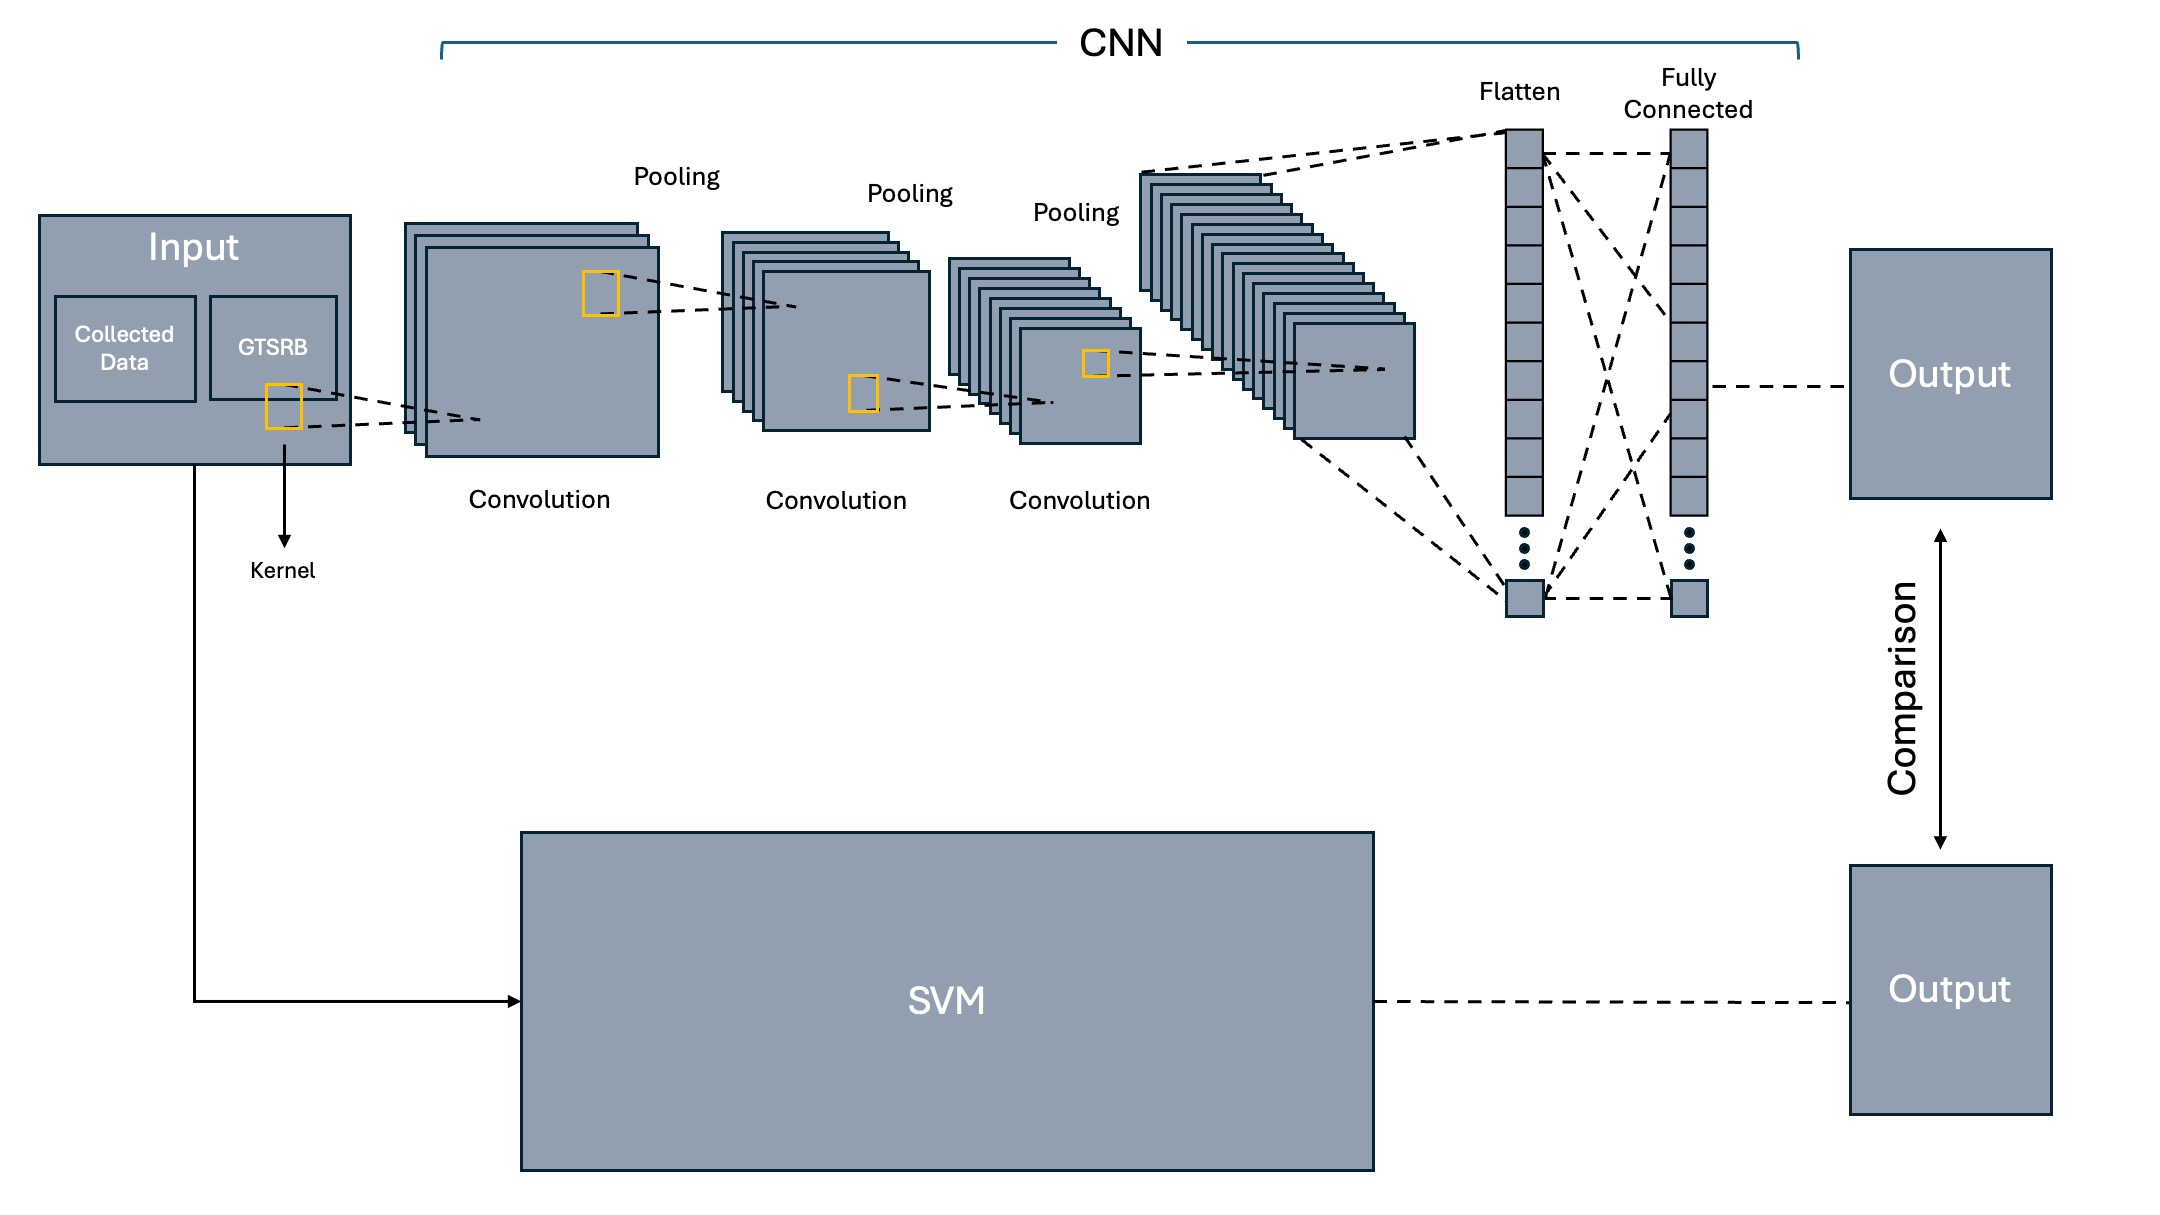
\includegraphics[width=\textwidth]{Figs/aps350_proposal_figure.jpg}
\end{center}
\caption{Diagram of proposed model.}
\end{figure}




\section{Ethical Considerations}
\subsection*{Bias}
\begin{itemize}
    \item Geographical and cultural bias: Traffic signs vary across different regions, countries and continents. Thus, it is important to choose a particular region to base the model on, and feed data exclusive to that region to increase the accuracy of the model and avoid confusion.
    \item Socioeconomic bias: The training data must contain a mix of signs from both higher and lower income areas to eliminate bias and ensure that the model can identify different signs regardless of socioeconomic status.
\end{itemize}
\subsection*{Privacy Concerns}
\begin{itemize}
    \item Data collection: Collection of data must be done carefully to ensure that no faces or license plates are accidentally captured and used. This is done to ensure that there is no breach in privacy.
\end{itemize}

\subsection*{Accuracy and Safety}
\begin{itemize}
    \item Testing in diverse environments: The testing data must include various different urban and rural environments to ensure that the model has seen and is able to classify signs with satisfactory accuracy regardless of the surrounding environments.
\end{itemize}
\newpage


\section{Project Plan}

\begin{table} [h]
    \centering
    \begin{tabular}{|p{2.1cm}|p{2.5cm}|p{2.5cm}|p{2.5cm}|p{2.5cm}|p{1.3cm}|} \hline 
    
         Task&  Maryah&  Sally&  Maya&  Member 4& Deadline\\ \hline 
         \multicolumn{6}{|c|}{Phase 1: Project Setup \& Data Collection}\\ \hline 
         
         Data collection \& preprocessing&  Download dataset, perform cleaning \& augmentation&  Review dataset, assist with data splitting (train/val/test)&  Compile list of universal traffic signs&  Help with augmentation strategies& Oct 13\\ \hline 
         Toronto Data Collection&  Collect 50 photos of various traffic signs&  Collect 50 photos of various traffic signs&  Collect 50 photos of various traffic signs&  Collect 50 photos of various traffic signs& Oct 13\\ \hline 
         \multicolumn{6}{|c|}{Phase 2: Baseline Model \& Initial Training}\\ \hline 
         Build the baseline model&  Assist with model setup&  Implement baseline CNN&  Assist with training baseline model&  Help with baseline evaluation setup (metrics, confusion matrix)& Oct 20\\ \hline 
         Evaluate the baseline model&  Help analyze dataset weaknesses (e.g. underfitting)&  Analyze model performance, document findings&  Help measure baseline performance (accuracy, confusion)&  Refine data (augmentation, cleaning)& Oct 25\\ \hline 
         \multicolumn{6}{|c|}{Phase 3: Model Optimization \& Hyperparameter Tuning}\\ \hline 
         Hyperparameter tuning&  Assist with tuning (learning rate, batch size)&  Focus on tuning regularization \& dropout rate&  Focus on tuning model complexity (layer depth, optimizers)&  Assist with experimentation (e.g., batch size, tuning)& Nov 10\\ \hline 
 Implement strategies to handle overfitting& Apply data augmentation (rotations, flips, zooms)& Add dropout layers to the architecture, tune dropout rate& Apply L2 regularization (weight decay) to control overfitting& Implement early stopping for the training process&Nov 13\\ \hline 
 Improve model architecture& Support advanced model experimentation& Test different architectures (residuals, deeper CNNs)& Implement advanced architectures or transfer learning& Assist with architecture analysis&Nov 15\\ \hline 
 \multicolumn{6}{|c|}{Phase 4: Evaluation \& Testing}\\ \hline 
 Model evaluation on test set& Run final accuracy metric on test set, compute overall accuracy& Evaluate model performance, interpret results (precision/recall)& Generate final confusion matrix and accuracy report& Document final accuracy, assist with report&Nov 19\\ \hline 
 \multicolumn{6}{|c|}{Phase 5: Documentation \& Presentation}\\ \hline 
         Prepare final report and presentation&  Write report sections (intro, dataset)&  Write methodology and model architecture sections&  Write result analysis section&  Write challenges, conclusion, and compile report& Nov 23\\ \hline
    \end{tabular}
    
    \caption{Project Plan and Task Delegation}
    \label{tab:my_label}
\end{table}

The tasks necessary to complete this project have been outlined and delegated, as shown in Table 1. We will collaborate by holding regular meetings every Thursday at 2PM, where we will review progress, discuss challenges, and plan upcoming tasks. To ensure consistent communication, we will utilize a dedicated group chat for daily updates, quick decisions, and clarifications. For seamless code collaboration, we will maintain a shared GitHub repository where all members can contribute. To avoid code overwriting, we will follow version control best practices, including using branches for individual tasks, submitting pull requests for review, and updating the team on active work to ensure synchronization.

\section{Risk Register}
\subsection{Data Overfitting}
Overfitting occurs in machine learning when a model accounts for the noise and outliers of its training data to an extent which negatively affects its performance on new data. This commonly occurs when there is an insufficient amount of data diversity. 

Likelihood: Medium

\subsubsection*{Resolution:}
\begin{itemize}
    \item Utilize data augmentation in order to vary image color, rotation, or scale to artificially expand the data set 
    \item Track validation loss so we can catch overfitting early on in order to adjust the training accordingly 
\end{itemize}
\subsection{Limited Data Diversity}
While the model will be tested with a selected dataset that is comprehensive, it is possible that it will not account for all possible variations of traffic signs encountered in real-world situations. This may result in the model failing to effectively generalize the data.  
\subsubsection*{Resolution:}
\begin{itemize}
    \item Use multiple datasets from different regions or create our own dataset
    \item Evaluate the model on real-life traffic signs collected from personal photos
    \item Attempt to use datasets with diverse conditions such as varying weather conditions, lighting, angles, etc.
\end{itemize}

\subsection{Model Training Duration}
The training for a model can be a time-consuming process when the architecture is complex or if the training data is large. This may result in project delays. 

Likelihood: Medium
\subsubsection*{Resolution}
\begin{itemize}
    \item Attempt to optimize system by modifying hyperparameters, simplifying model complexity, or use more efficient algorithms in order to speed up the training process
    \item Set a time limit for training runs and monitor validation performance to stop training when performance plateaus to avoid unnecessary system cost
    \item Add checkpoints to save intermediate models in case of losing progress due to long runs or run fails
\end{itemize}

\subsection{Team Member Dropout}
The possibility of a team member dropping the course will result in disruptions in the project process and workload distribution.

Likelihood: Low
\subsubsection*{Resolution}
\begin{itemize}
    \item Ensure multiple team members are training in important tasks, so that if in the case of a team member leaving, there will be a smooth transition of tasks
    \item Maintain a comprehensive documentation of the project progress and process to help teammates who take on additional tasks
\end{itemize}

\section{Github Link}
https://github.com/sysallykim/aps360\_fall2024\_group28

\section{References}

\label{last_page}

\bibliography{APS360_ref}
\bibliographystyle{iclr2022_conference}

\end{document}
